
\section{程序说明}

\begin{figure}[H]
    \begin{center}
        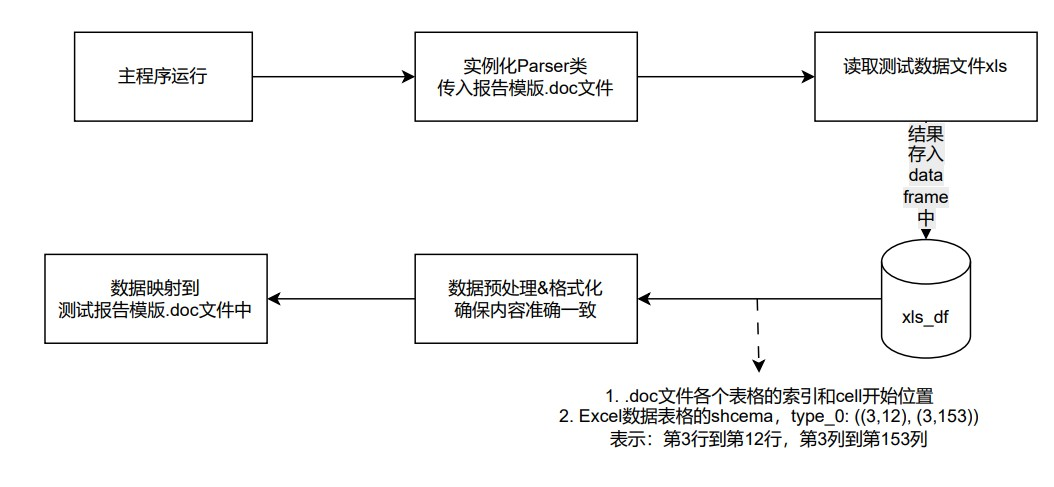
\includegraphics[width=.95\linewidth]{res/autotable.jpg}\\
        \caption{autotable program running flowchart}\label{autotable}
    \end{center}
\end{figure}

\subsection{报告模板解析}
测试报告模版如下:
\vspace{-.7cm}
    \begin{itemize}
        \item 三相智能电表测试报告模版:\texttt{IEC20-三相四线-报告输出\_3p.docx}  % 下划线需要转义
        \item 单相智能电表双回路测试报告模版:IEC20-单相两线-双回路-报告输出\_1p.docx % 和上面意思一样,只要将下划线转义
        \item 其它模版,未实现.......
    \end{itemize}

测试报告模版表格索引和cell定位(由于测试报告格式不会经常变,综合考虑,通过人工方式将word模版的表格index和cell的起始定位找出,写入parquet文件中)
\begin{figure}[H]
    \begin{center}
        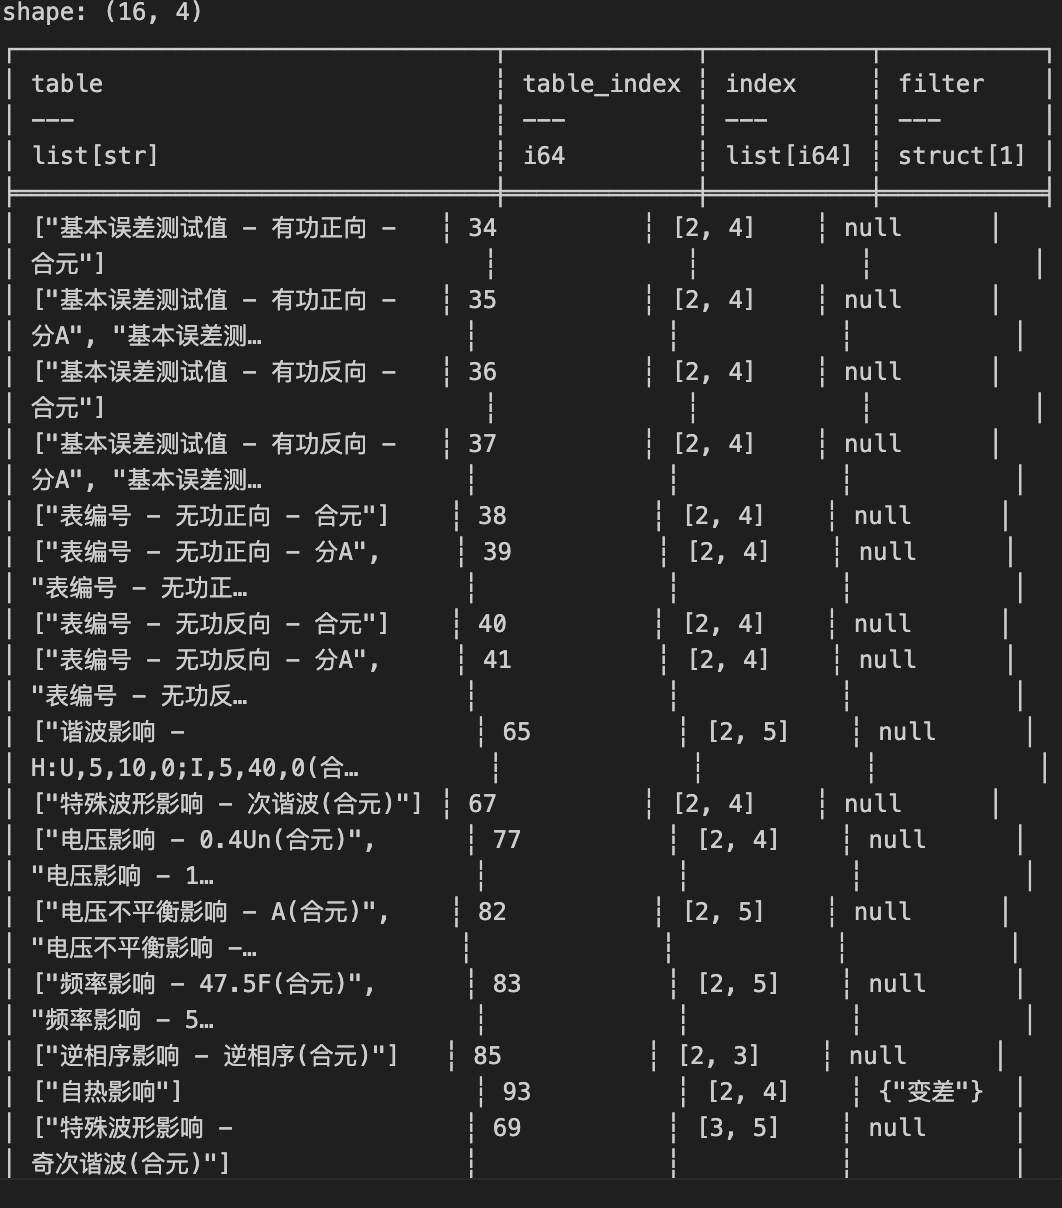
\includegraphics[width=.95\linewidth]{res/3p_parquetdata.png}\\
        \caption{indexref\_3p.parquet 文件内容 }\label{3p_parquetdata}
    \end{center}
\end{figure}

indexref\_1p.parquet \hspace{0.4em}  \faArrowRight \hspace{0.4em} IEC20-单相两线-双回路-报告输出\_1p.docx\\
indexref\_3p.parquet \hspace{0.4em} \faArrowRight \hspace{0.4em} IEC20-三相四线-报告输出\_3p.docx\\


\subsection{数据模板解析}
测试数据模版如下:
\vspace{-.7cm}
    \begin{itemize}
        \item 三相智能电表测试数据模版:\texttt{IEC20-三相四线-瑞科台子-计量误差数据.xls} 
        \item 单相智能电表双回路测试数据模版:IEC20-单相两线-双回路-瑞科台子-计量误差数据 
        \item 其它模版,未实现.......
    \end{itemize}

读取excel数据时,表格schema设计如下:
\begin{figure}[H]
    \begin{center}
        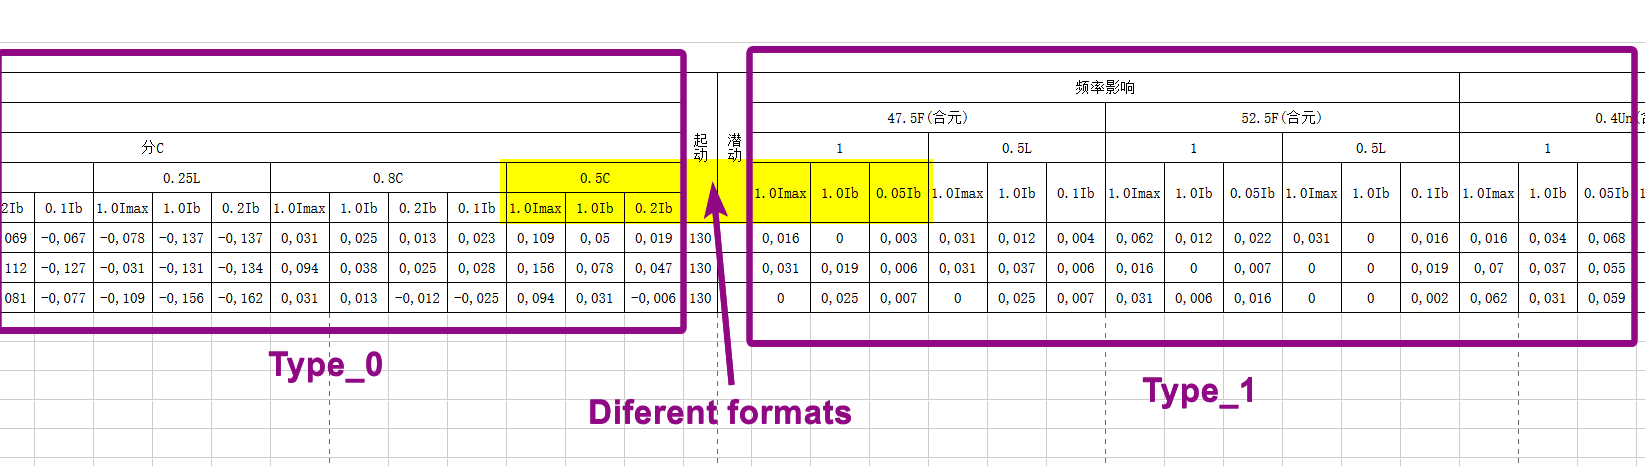
\includegraphics[width=.95\linewidth]{res/excel_type.png}\\
        \caption{Different table type }\label{excel_type}
    \end{center}
\end{figure}

以 \textbf{IEC20-三相四线-瑞科台子-计量误差数据.xls} 数据模版为例,读取此文件时的shcema如下:

\[ 
schema= \left\{
\begin{array}{ll}
    'type_0': ((3, 12), (3, 153)),\\
    'type_1': ((3, 12), (155, -7)),\\
    'type_2': ((3, 12), (190, -1)),\\
    'type_3': ((3, 12), (3, 153))\\
\end{array} 
\right. 
\]

\subsection{常用修改命令}

如何修改parquet文件中的内容,举例:

\begin{minted}[frame=lines,framesep=1mm]{python}
# read parquet file
parquet_file = "indexref_3p.parquet"
print("\n从Parquet文件读取验证:")
df = pl.read_parquet(parquet_file)

# modify the DataFrame
df = df.with_columns(
    pl.when(pl.col('table_index').eq(78)) #条件判断,判断table_index是否等于78
    .then(pl.lit(['modified']))  #如果条件满足,则将'table'列的值修改为'modified'
    .otherwise(pl.col('table')) #否则保持原来的'table'列的值
    .alias('table')  #重命名列为'table'
)
\end{minted}

修改前后对比:

\begin{figure}[H]
    \begin{center}
        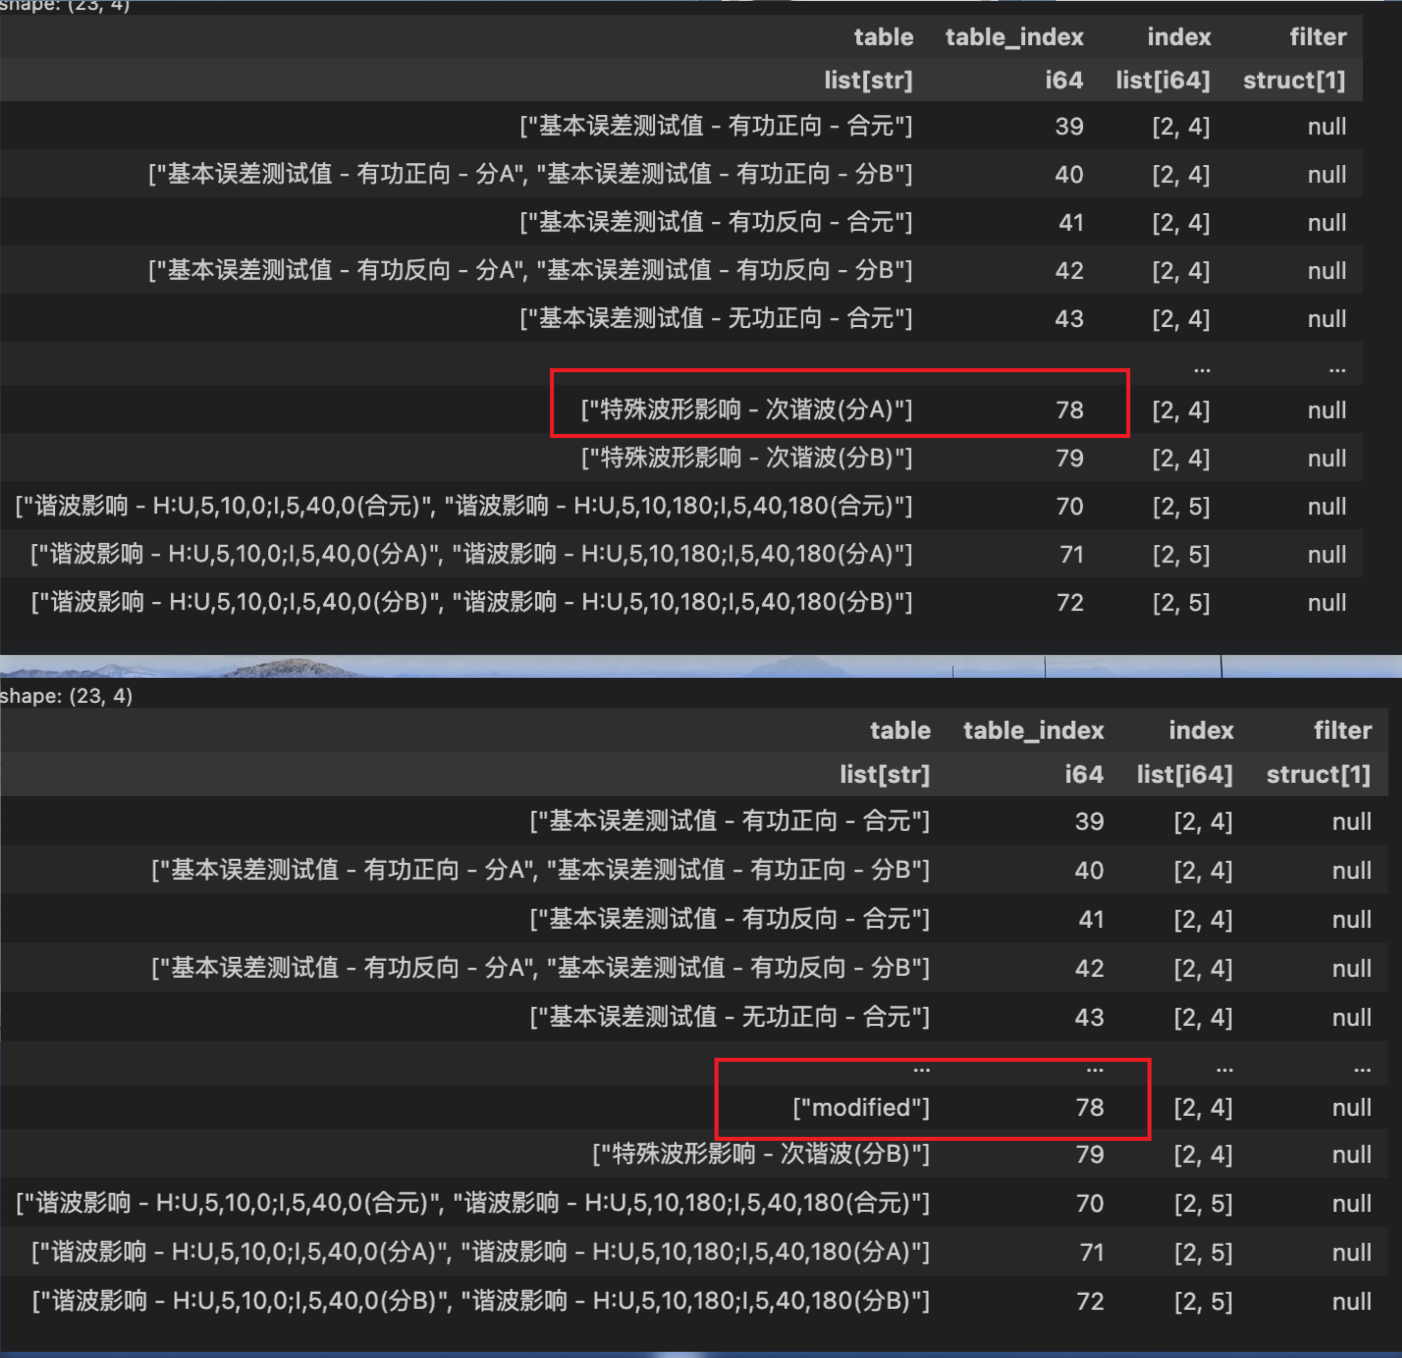
\includegraphics[width=.95\linewidth]{res/modify.png}\\
        \caption{数据修改前后对比}\label{modify}
    \end{center}
\end{figure}

\section{写在后面}

时间仓促,目前只完成部分功能,未能做通用适配和界面化工作,后续可提升。
感谢Lucas Costa对此项目的突出贡献!

% \vspace{-.7cm}
    \begin{itemize}
        \item 将此程序作为服务端,实现B/S模式,客户端直接浏览器操作,可视化。
        \item 此程序在映射数据时,目前只针对模板内容,进行3只表处理,后面要能处理可配置数量的电能表。 
        \item 主程序中,未做批处理循环操作,可结合第一条,选择目录循环处理,一次处理多个报告模板和数据。
    \end{itemize}

%\section{实验}
%\subsection{实验设置}
%设置实验环境、实验指标、对比方法等。
